\documentclass{beamer}
\usepackage{ragged2e}   % Package for justification
\usepackage[utf8]{inputenc}
\usepackage[english]{babel}
\usepackage[T1]{fontenc}
\usepackage{helvet}

% To print page number and footer
\setbeamertemplate{footline}[text line]{
  \parbox{\linewidth}{\vspace*{-8pt}Mr. Harish D. Gadade\hfill\insertshortauthor\hfill\insertpagenumber}}
\setbeamertemplate{navigation symbols}{}
\author[Govt. Colleg of Engg, Jalgaon]{}
% End Page number and footer

% To pring Header
%\setbeamertemplate{headline}{%
%\leavevmode%
 % \hbox{%
  %  \begin{beamercolorbox}[wd=\paperwidth,ht=2.5ex,dp=1.125ex]{palette quaternary}%
   % \insertsectionnavigationhorizontal{\paperwidth}{}{\hskip0pt plus1filll}
    %\end{beamercolorbox}%
 % }
%}
%End Header

% Logo do canto inferior direito
%\pgfdeclareimage[height=0.7cm]{gcoejLogo}{gcoejLogo}
\pgfdeclareimage[height=1cm]{gcoejLogo}{gcoejLogo}
\logo{
	\vspace*{8.2cm}
	%\vspace*{-0.25cm}
	\pgfuseimage{gcoejLogo}
	\hspace*{-0.05cm}}
	%\hspace*{-0.05cm}}



\begin{document}
\section{DSM}
\begin{frame}
	\centering
	\large Unit-IV\\
	\huge{Distributed Shared Memory}\\ 
	\vspace{2cm}
	\small{Mr.Harish D. Gadade}\\
	\small{Govt. College of Engg., Jalgaon}
\end{frame}


\subsection{Architecture of DSM}
\begin{frame}
	\frametitle{General Architecture of DSM Systems}
	\begin{figure}
	 	\centering
	 	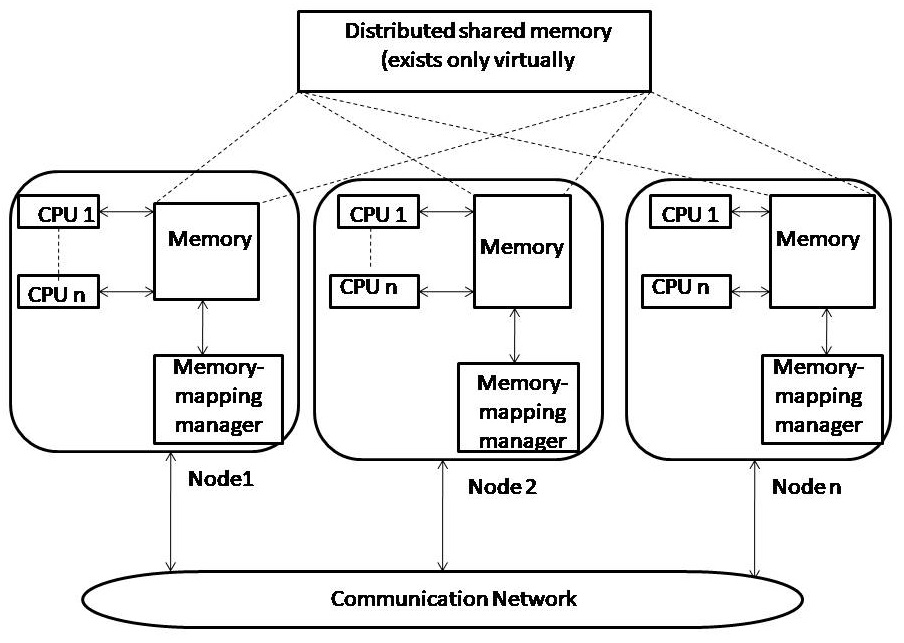
\includegraphics[width=10cm]{fig51.jpg}
	 	\caption{Distributer Shared Memory}\label{fig51}
	 \end{figure}
\end{frame}


\subsection{Implementation Issues}
\begin{frame}
	\frametitle{Design and Implementation Issues of DSM}
	Important Issues involved in the design and implementation of DSM system are;
	\begin{enumerate}
		\item \textit{Granularity}
		\item \textit{Structure and Shared Memory Space}
		\item \textit{Memory Coherence and Access Synchronization}
		\item \textit{Data Location and Access}
		\item \textit{Replacement Strategy}
		\item \textit{Trashing}
		\item \textit{Heterogeneity}
	\end{enumerate}
	\vspace{2cm}
\end{frame}

\subsection{Granularity}
\begin{frame}
	\frametitle{Granularity}
	\justifying {One of the most visible parameters to be chosen in the design of a DSM system is the \underline {Block Size}. Several criteria for 
	choosing this granularity parameter are described as;}\\
	\vspace{0.5cm}
	\textbf{1. Factors Influencing Block Size Selection}\\
	\vspace{0.5cm}
	Factors that influence the choice of block size are;
	\vspace{0.25cm}
	\begin{enumerate}
		\item \textit{Paging Overhead}
		\item \textit{Directory Size}
		\item \textit{Trashing}
		\item \textit{False Sharing}
	\end{enumerate}
	\vspace{2cm}
\end{frame}


\begin{frame}
	\frametitle{Granularity...[Cntd...]}
	\begin{figure}
	 	\centering
	 	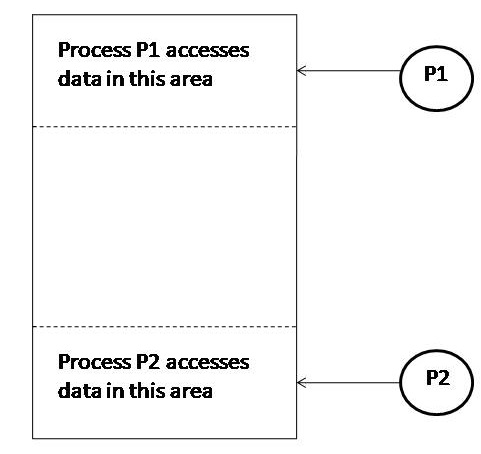
\includegraphics[width=6cm]{fig52.jpg}
	 	\caption{False Sharing}\label{fig52}
	 \end{figure}

\end{frame}


\begin{frame}
	\frametitle{Granularity...[Cntd...]}
	\textbf{2. Using Page Size as Block Size}\\
	\vspace{0.5cm}
	Using page size as the block size of a DSM has the following advantages;
	\vspace{0.5cm}
	\begin{enumerate}
		\item \textit{Page Fault Handler}
		\item \textit{It allows the access right control to be readily integrated into functionality of the memory management unit of the system.}
		\item \textit{As long as a page cant into a packet, page size do not impose undue communication overhead at the time of network page fault.}
		\item \textit{Experiences has shown that a page size is a suitable data entity unit with respect to memory contention.}
	\end{enumerate}
\end{frame}


\begin{frame}
	\frametitle{Structure of Shared-Memory Space}
	The three commonly used approaches for structuring the shared memory space of a DSM are;
	\vspace{0.5cm}
	\begin{enumerate}
		\item \textit{No Structuring}
		\item \textit{Structuring by data type}
		\item \textit{Structuring as a database}
	\end{enumerate}
	\vspace{4cm}
\end{frame}


\begin{frame}
	\frametitle{Consistency Models}
	\vspace{0.5cm}
	\begin{enumerate}
		\item \textit{Strict Consistency Model}
		\item \textit{Sequential Consistency Model}
		\item \textit{Causal Consistency Model}
		\item \textit{Pipelined Random-Access Memory Consistency Model}
		\item \textit{Processor Consistency Model}
		\item \textit{Weak Consistency Model}
		\item \textit{Release Consistency Model}
		\item \textit{Discussion of Consistency Model}
	\end{enumerate}
	\vspace{4cm}
\end{frame}


\begin{frame}
	\frametitle{Implementation of Sequential Consistency Model}
	\vspace{0.5cm}
	The Designer of DSM system may choose from among the following replication and migration strategies
	\vspace{0.5cm}
	\begin{enumerate}
		\item \textit{Nonreplicated, Nonmigrating Block(NRNMBs)}
		\item \textit{Nonreplicated, Migrating Blocks(NRMBs)}
		\item \textit{Replicated, Migrating Blocks(RMBs)}
		\item \textit{Replicated, Nonmigrating Blocks(RNMBs)}
	\end{enumerate}
	\vspace{4cm}
\end{frame}


\begin{frame}
	\frametitle{1.Nonreplicated, Nonmigrating Block(NRNMBs)}
	\begin{figure}
		\centering
		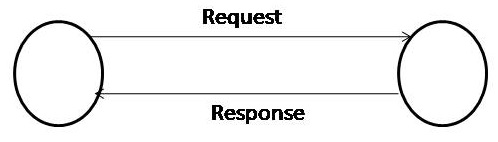
\includegraphics[width=4cm]{fig53.jpg}
		\caption{Nonreplicated, Nonmigrating Block(NRNMB) Strategy}
		\label{fig53}
	\end{figure}
	\underline{Drawbacks}
	\vspace{0.25cm}
	\begin{itemize}
		\item \textit{Serializing data access creates a bottleneck}
		\item \textit{Parallelism, which is a major advantage of DSM, is not possible with this method}
	\end{itemize}
	\underline{Data Locating in NRNMB Strategy:}
	\vspace{0.25cm}
	\begin{itemize}
		\item \textit{There is a single copy of each block in the entire system}
		\item \textit{The location of a block never changes}
	\end{itemize}
\end{frame}


\begin{frame}
	\frametitle{2.Nonreplicated,Migrating Block}
	\begin{figure}
		\centering
		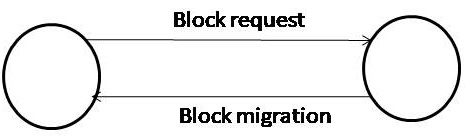
\includegraphics[width=4cm]{fig54.jpg}
		\caption{Nonreplicated, Migrating Block Strategy}
		\label{fig54}
	\end{figure}
	\underline{Advantages}
	\vspace{0.25cm}
	\begin{itemize}
		\item \textit{No communication costs are incurred when a process accesses data currently held locally.}
		\item \textit{It allows the applications to take advantage of data access locally.}
	\end{itemize}
	\underline{Disadvantages:}
	\vspace{0.25cm}
	\begin{itemize}
		\item \textit{It is prone to thrashing problem}
		\item \textit{The advantage of parallelism cannot be availed in this method also.}
	\end{itemize}
\end{frame}


\begin{frame}
	\frametitle{2.Nonreplicated,Migrating Block...[Cntd...]}
	\underline{Data Locating in the NRMB Strategy:}\\
	\vspace{0.25cm}
	One of the following methods may be used in this strategy to locate a block
	\vspace{0.25cm}
	\begin{enumerate}
		\item \textit{Broadcasting}
		\item \textit{Centralized-Server Algorithm}
		\item \textit{Fixed Distributed-Server Algorithm}
		\item \textit{Dynamic Distributed-Server Algorithm}
	\end{enumerate}
	\vspace{2cm}
\end{frame}



\begin{frame}
	\frametitle{2.Nonreplicated,Migrating Block...[Cntd...]}
	\underline{1. Broadcasting}
	\vspace{0.25cm}
	\begin{figure}
		\centering
		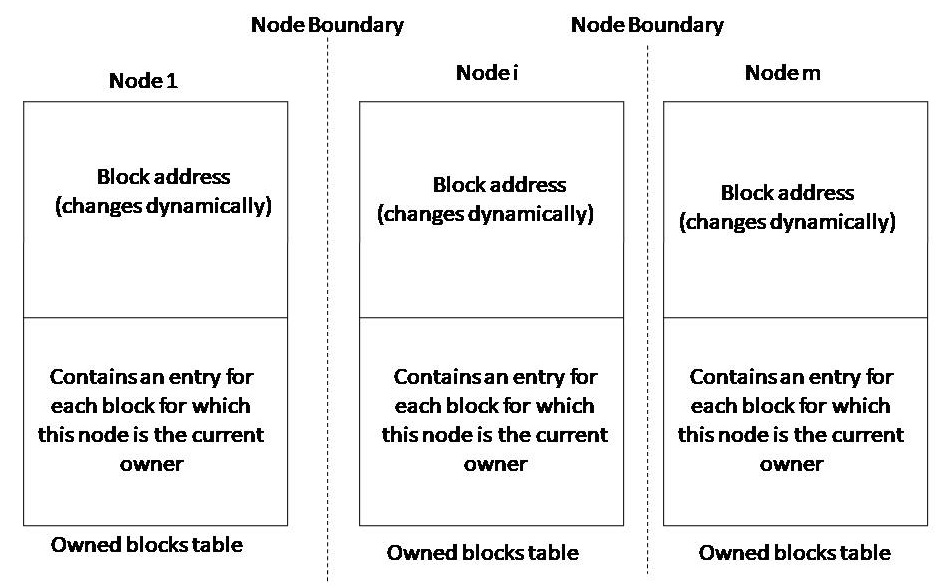
\includegraphics[width=8cm]{fig55.jpg}
		\caption{Structure and Location of owned blocks table in the Broadcasting Data Locating Mechanism for NRMB Strategy}
		\label{fig55}
	\end{figure}
\end{frame}


\begin{frame}
	\frametitle{2.Nonreplicated,Migrating Block...[Cntd...]}
	\underline{2. Centralized-Server Algorithm}
	\vspace{0.25cm}
	\begin{figure}
		\centering
		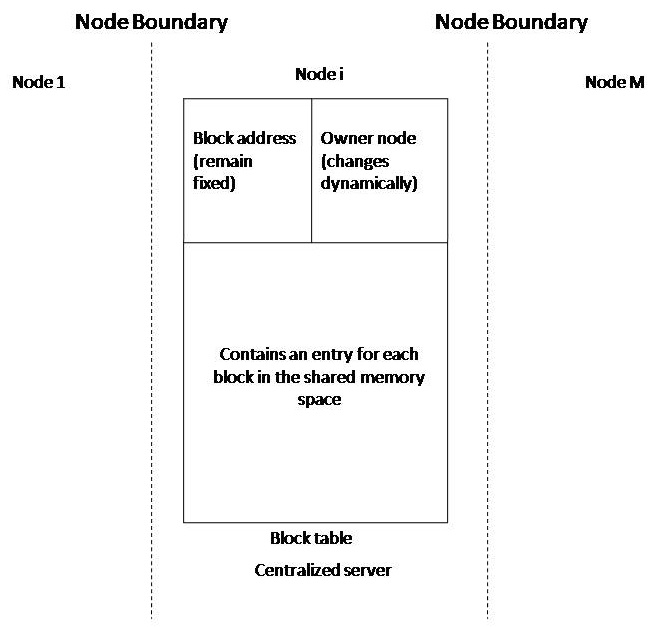
\includegraphics[width=6cm]{fig56.jpg}
		\caption{Structure and Location of block table in the Centralized-Server Data Locating Mechanism for NRMB Strategy}
		\label{fig56}
	\end{figure}
\end{frame}


\begin{frame}
	\frametitle{2.Nonreplicated,Migrating Block...[Cntd...]}
	\underline{3. Fixed Distributed-Server Algorithm}
	\vspace{0.25cm}
	\begin{figure}
		\centering
		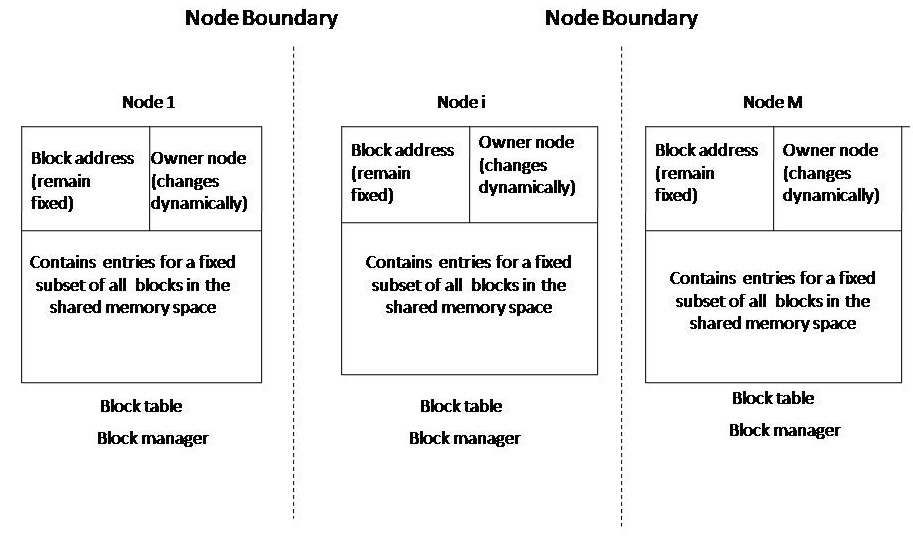
\includegraphics[width=8cm]{fig57.jpg}
		\caption{Structure and Location of owned blocks table in the Fixed Distributed-Server Data Locating Mechanism for NRMB Strategy}
		\label{fig57}
	\end{figure}
\end{frame}

\begin{frame}
	\frametitle{2.Nonreplicated,Migrating Block...[Cntd...]}
	\underline{4. Dynamic Distributed-Server Algorithm}
	\vspace{0.25cm}
	\begin{figure}
		\centering
		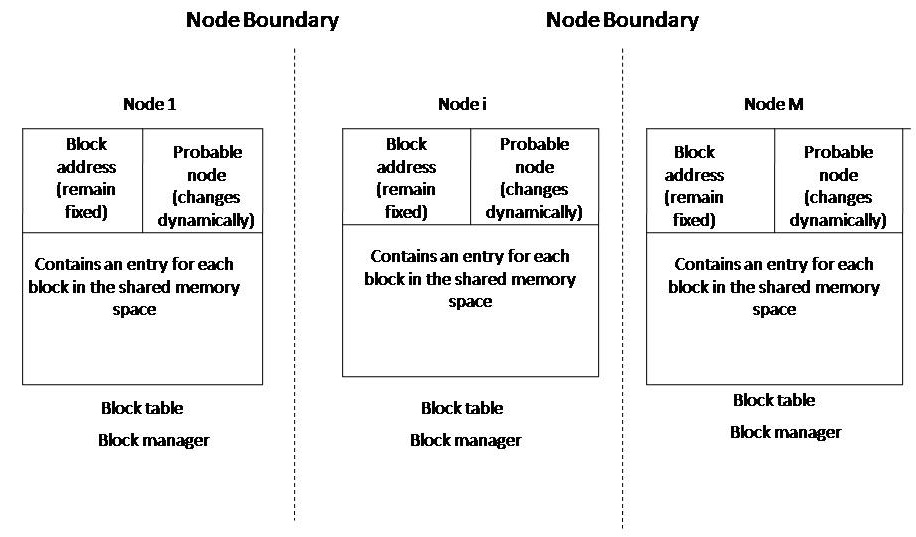
\includegraphics[width=8cm]{fig58.jpg}
		\caption{Structure and Location of owned blocks table in the Dynamic Distributed-Server Data Locating Mechanism for NRMB Strategy}
		\label{fig58}
	\end{figure}
\end{frame}


\begin{frame}
	\frametitle{3.Replicated, Migrating Blocks}
	The two basic protocols that may be used for ensuring sequential consistency
	\vspace{0.25cm}
	\begin{itemize}
		\item Write-Invalidate
	\end{itemize}
	\begin{figure}
		\centering
		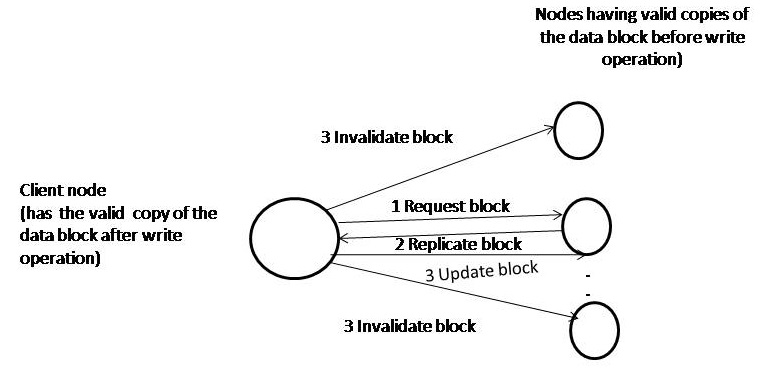
\includegraphics[width=10cm]{fig59.jpg}
		\caption{Write-Invalidate memory approach for RMB strategy}
		\label{fig59}
	\end{figure}
\end{frame}


\begin{frame}
	\frametitle{3.Replicated, Migrating Blocks...[Cntd...]}
	\vspace{0.25cm}
	\begin{itemize}
		\item Write-Update
	\end{itemize}
	\begin{figure}
		\centering
		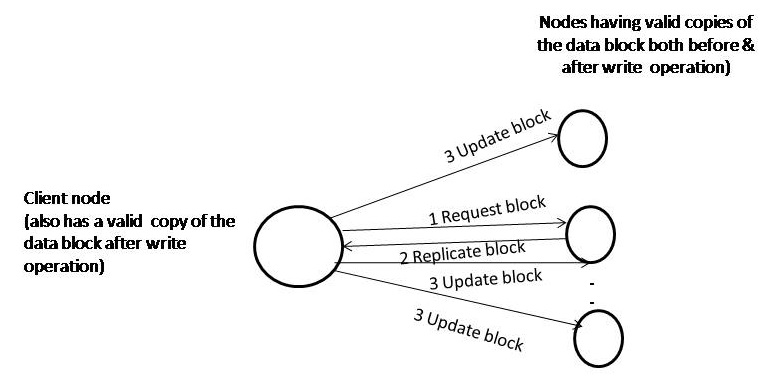
\includegraphics[width=10cm]{fig510.jpg}
		\caption{Write-Update memory approach for RMB strategy}
		\label{fig510}
	\end{figure}
\end{frame}


\begin{frame}
	\frametitle{3.Replicated, Migrating Blocks...[Cntd...]}
	\vspace{0.25cm}
	\underline{Data Locating in RNM Strategy}\\
	\vspace{0.5cm}
	The following data locating issues are involved in the Write-Invalidate protocol used with RMB strategy
	\begin{itemize}
		\item \textit{Locating the owner of the block}
		\item \textit{Keeping track of the node that currently have a valid copy of the block}
	\end{itemize}
	One of the following algorithms may be used to address these two issues\\
	\begin{enumerate}
		\item \textit{Broadcasting}
		\item \textit{Centralized-Server Algorithm}
		\item \textit{Fixed Distributed-Server Algorithm}
		\item \textit{Dynamic Distributed-Server Algorithm}
	\end{enumerate}
\end{frame}


\begin{frame}
	\frametitle{3.Replicated, Migrating Blocks...[Cntd...]}
	\vspace{0.25cm}
	\underline{1. Broadcasting}
	\begin{figure}
		\centering
		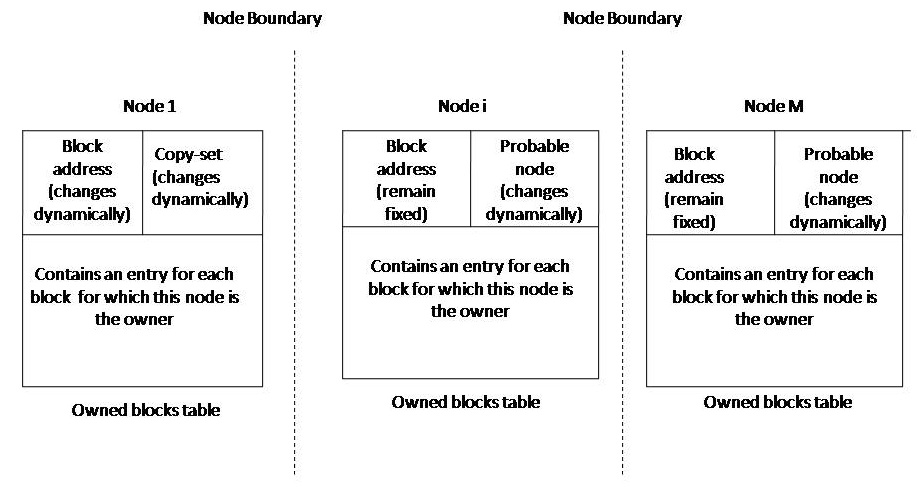
\includegraphics[width=10cm]{fig512.jpg}
		\caption{Structure and Location of owned blocks table in the broadcasting Data Locating Mechanism for RMB Strategy}
		\label{fig512}
	\end{figure}
\end{frame}


\begin{frame}
	\frametitle{3.Replicated, Migrating Blocks...[Cntd...]}
	\vspace{0.25cm}
	\underline{2. Centralized-Server Algorithm}
	\begin{figure}
		\centering
		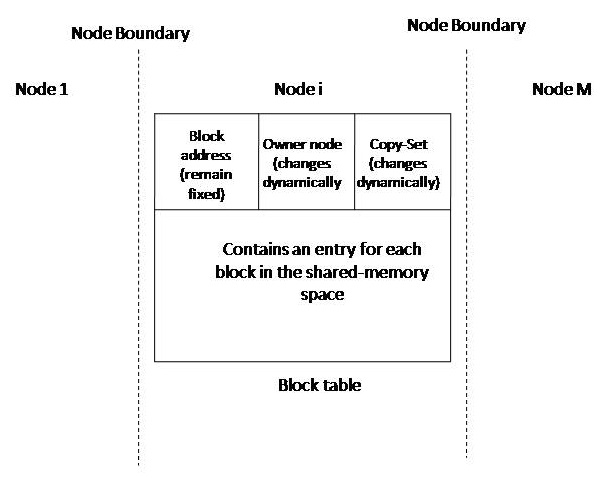
\includegraphics[width=8cm]{fig513.jpg}
		\caption{Structure and Location of owned blocks table in the Centralized-Server Data Locating Mechanism for RMB Strategy}
		\label{fig513}
	\end{figure}
\end{frame}


\begin{frame}
	\frametitle{3.Replicated, Migrating Blocks...[Cntd...]}
	\vspace{0.25cm}
	\underline{3. Fixed Distributed-Server Algorithm}
	\begin{figure}
		\centering
		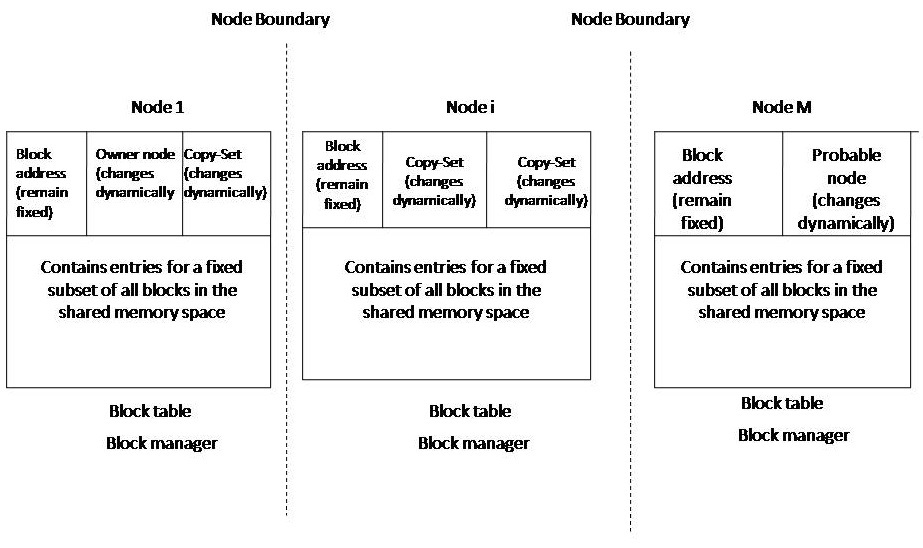
\includegraphics[width=10cm]{fig514.jpg}
		\caption{Structure and Location of blocks table in the fixed distributed Server Data Locating Mechanism for RMB Strategy}
		\label{fig514}
	\end{figure}
\end{frame}

\begin{frame}
	\frametitle{3.Replicated, Migrating Blocks...[Cntd...]}
	\vspace{0.25cm}
	\underline{4. Dynamic Distributed-Server Algorithm}
	\begin{figure}
		\centering
		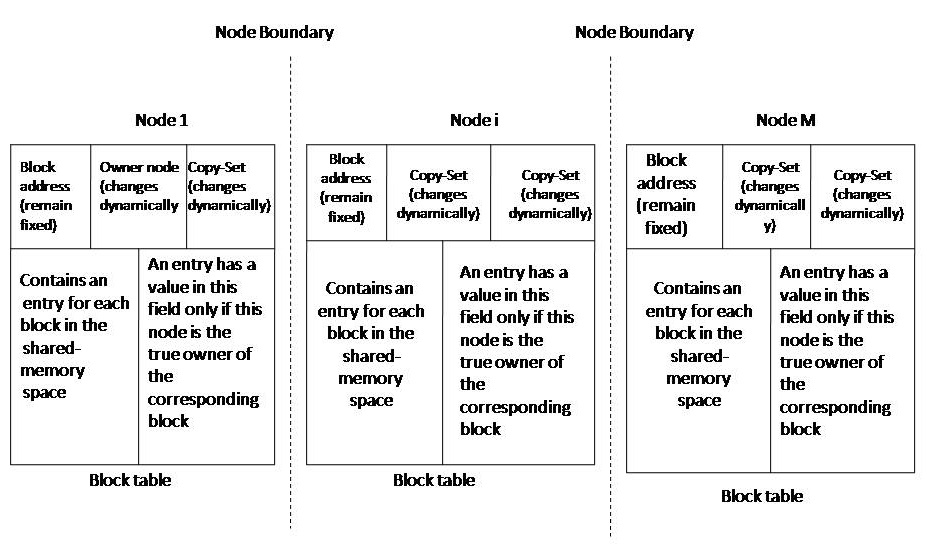
\includegraphics[width=10cm]{fig515.jpg}
		\caption{Structure and Location of blocks table in the Dynamic distributed Server Data Locating Mechanism for RMB Strategy}
		\label{fig515}
	\end{figure}
\end{frame}


\begin{frame}
	\frametitle{4.Replicated, Migrating Blocks}
	\justifying{In this strategy, a shared memory block ma be replicated at multiple nodes of the system but the location of each replica is fixed. A read 
	or write access to a memory address is carried out by sending the process request to one of the nodes having replica of the block containing the memory 
	address.}\\
	\vspace{0.5cm}	
	\underline{Data Locating in the RNMB Strategy}\\
	\vspace{0.25cm}
	The RNMB strategy has following caracteristics
	\vspace{0.25cm}
	\begin{enumerate}
		\item \textit{The replica location of a block never change}
		\item \textit{All replica of a data blocks are kept consistent}
		\item \textit{Only a read request can be directly sent to one of the nodes having a replica of the blocks.}
	\end{enumerate}
\end{frame}


\begin{frame}
	\frametitle{4.Replicated, Migrating Blocks...[Cntd...]}
	\begin{figure}
		\centering
		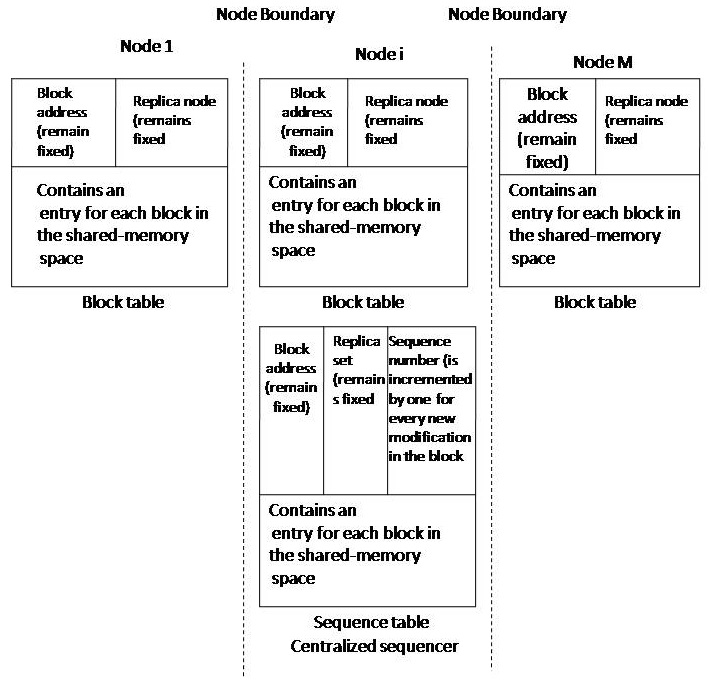
\includegraphics[width=8cm]{fig516.jpg}
		%\caption{Structure and Location of blocks table in the Dynamic distributed Server Data Locating Mechanism for RMB Strategy}
		\label{fig516}
	\end{figure}
\end{frame}


\begin{frame}
	\frametitle{Replacement Strategy}
	\justifying{DSM system that allows shared memory blocks to be dynamically migrated/replicated. Following issues must be addressed when the available 
	space for catching shared data fills up at a node;.}\\
	\vspace{0.5cm}	
	\begin{itemize}
		\item \textit{Which Block to Replace}
		\item \textit{Where to Place a Replaced Block}
	\end{itemize}
	\vspace{2cm}
\end{frame}


\begin{frame}
	\frametitle{Heterogeneous DSM}
	\justifying{Two main issues in the building a DSM system on a network of heterogeneous machines are;.}\\
	\vspace{0.5cm}	
	\begin{itemize}
		\item \textit{Data Conversion}
		\item \textit{Block Size Selection}
	\end{itemize}
	\vspace{2cm}
\end{frame}


\begin{frame}
	\frametitle{Advantages of DSM}
	\vspace{0.5cm}	
	\begin{itemize}
		\item \textit{Simple Abstraction}
		\item \textit{Better Probability of Distributed Application Programs}
		\item \textit{Better Performance of some Application}
		\item \textit{Flexible Communication Environment}
		\item \textit{Ease of Process Migration}
	\end{itemize}
	\vspace{4cm}
\end{frame}


\end{document}